Power Automate ist ein Teil der Microsoft Power-Platform, mit der man Cloud-basierte Automatisierungsprozesse erstellen und verwalten kann. Der Benutzer hat Zugriff auf verschiedene Dienste von Microsoft und kann ohne oder wenig Code einen Workflow erstellen. Power Automate reagiert auf einen im Vorhinein definierten Trigger und führt eine Reihe von vordefinierten Schritten aus. Dieser Trigger kann eine neue E-Mail, ein neuer Datensatz im CRM eingefügt wird oder einfach die Erstellung eines neuen Dokuments im SharePoint sein. Somit ist es möglich auch ohne jegliche Vorkenntnisse oder fachspezifisches Wissen eine einfache Anwendung zu erstellen. Zum Beispiel kann beim Eingang einer E-Mail, die eine Kundenrechnung enthält, an den AI-Builder weitergegeben werden und dort mit einem vortrainierten Modell, die wichtigsten Daten herauslesen und dann erneut mit einer E-Mail versendet werden.

\subsection{Cloud Flow}
Da bei dieser Arbeit nur der Cloud Flow in Verwendung ist, wird hier nur auf diesen genauer eingegangen. Power Automate bietet hier drei verschiedene Arten von Cloud Flows an:

\begin{enumerate}
    \item Automated Flow
    \item Instant Flow
    \item Scheduled Flow
\end{enumerate}

\subsubsection{Automated Flow}
Dieser Flow wird ausgelöst, wenn eine gewünschte Kondition eintritt. Solche Trigger können, der Eingang einer E-Mail einer speziellen Person, eine Teams-Nachricht oder wenn ein Dokument in OneDrive geändert wird. Sogenannte Connectors werden verwendet, um eine Folge von Schritten zu bilden, um den gewünschten Effekt zu erzielen.

\subsubsection{Instant Flow}
Ein Instant Flow wird mit dem Klicken eines Buttons gestartet. Dieser Flow läuft sowohl auf Mobile als auch auf Desktop Devices. Er wird verwendet, um ein breites Spektrum von Aufgaben zu erledigen, wie die Beantragung einer Genehmigung via Teams oder SharePoint.

\subsubsection{Scheduled Flow}
Dieser Flow wird nach einem Zeitplan automatisiert und zu einem gewünschten Datum oder beliebiger Uhrzeit ausgeführt werden. Dieser Ablauf ist hilfreich, um zum Beispiel jeden Tag zur selben Uhrzeit einen Daten-Upload zu machen.

\subsubsection{Cloud Flow in der Praxis}
Die Diplomanden dieser Arbeit entschieden sich für einen Automated Flow, da dieser die gewünschte Funktion erfüllt. Wie bereits erwähnt, ist der Automated Flow ein Event-basierter Flow und wird durch das Erhalten einer E-Mail ausgelöst (Siehe Abbildung \ref{fig:flow-trigger}).

\begin{figure}[h]
    \centering
    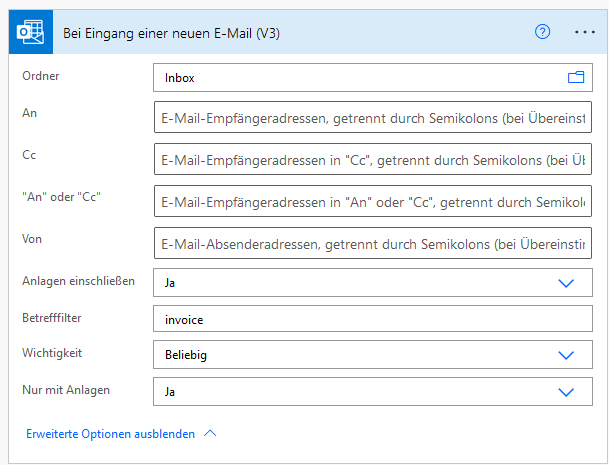
\includegraphics[scale=0.9]{sections/cloud-computing/images/power-automate-flow/trigger.png}
    \caption{Power Automate Flow Trigger}
    \label{fig:flow-trigger}
\end{figure}

Um alle Anlagen der E-Mail zu verarbeiten, wird eine Schleife um die nächsten Schritte gesetzt. Da es erlaubt ist mehrere Eingangsrechnungen in der E-Mail anzuhängen muss jeder Anhang einzeln verarveitet werden. Das zuvor definierte AI-Builder Modell extrahiert die notwendigen Information aus dem Dokument (Siehe Abbildung \ref{fig:ai-model-in-use}).

\begin{figure}[H]q
    \centering
    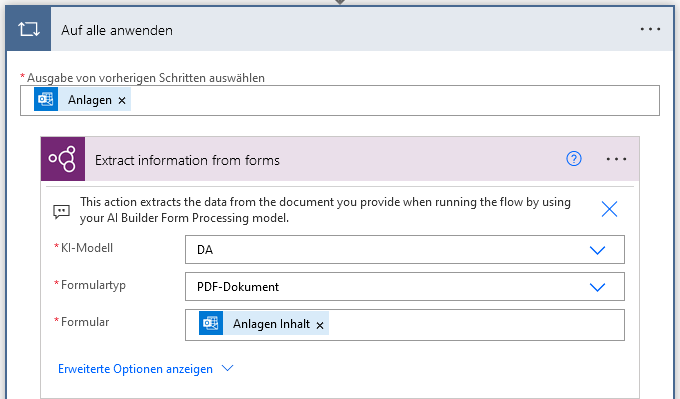
\includegraphics[scale=0.8]{sections/cloud-computing/images/power-automate-flow/ai-model-in-use.png}
    \caption{Verarbeitung des Dokuments}
    \label{fig:ai-model-in-use}
\end{figure}

Um die extrahierten Daten zu persistieren, wurde eine Dynamcis CRM Testumgebung aufgesetzt, um einen ecten Geschäftsfall zu simulieren. Es wurden zwei Entitäten, Invoice und Invoice Items erstellt (\ref{fig:class-diagram}). Da die Entität Invoice Items von der Entität Invoice abhängig ist, muss die die Entität Invoice Items eigens gespeichert werden.

\textbf{Kurzer Exkurs; Microsoft Dynamics CRM:}
Customer Relationship Management (CRM) beinhaltet eine Reihe von Software-Tools, die für das Verwalten der drei Pfeiler zwischen Kunde und Unternehmen zuständig sind: Marketing, Verkauf und Dienstleistungen. Neben Sammeln von Kudendaten aus verschiedenen Quellen und Automatisieren von sich wiederholenden Vertriebs-, Marketing- und Kundendienstprozessen, fördert eine CRM-Software auch die Abteilungsübergreifende Zusammenarbeit. Diese CRM-Software lässt sich in zwei Arten unterscheiden:
\begin{enumerate}
    \item On-Premise CRM-Software
    \item Cloud-basierte CRM-Software
\end{enumerate}

\subsubsection{On-Premise CRM-Software}
Da das Hauptgeschäft von Unternehmen wie Gesundheits- und Finanzeinrichtungen, der Umgang mit sensiblen Kundendaten ist, wird aus Sicherheitsgründen eine On-Premise Lösung, sprich eine CRM-Software vor Ort, bevorzugt. Diese Systeme sind aber mit hohen Wartungs- und Entwicklungskosten verbunden, und die Unternehmen sind selbst für Sicherheit und Datenpflege zuständig.  

\subsubsection{Cloud-basierte CRM-Software}
Unternehmen haben die Möglichkeit die CRM-Software und die damit verbundenen Aufwände, in die Cloud zu verlagern. Im Gegensatz du der On-Premise Lösung ist die Cloud-Variante flexibler in Hinsicht auf Speicher- und Rechenressourcen.

\begin{figure}[h]
    \centering
    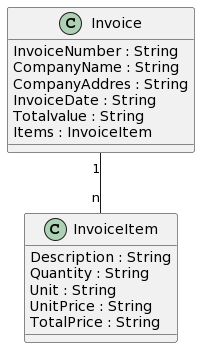
\includegraphics[scale=0.5]{sections/cloud-computing/images/power-automate-flow/cld.png}
    \caption{Klassendiagram Invoice}
    \label{fig:class-diagram}
\end{figure}

Um die Richtigkeit des Datenmodells zu sichern muss die Reihenfolge der Persistierung beachtet werden und alle Invoice Items abhängig von der dazugehörigen Invoice gemacht werden \ref{fig:persistence-entities}.

\begin{figure}[h]
    \centering
    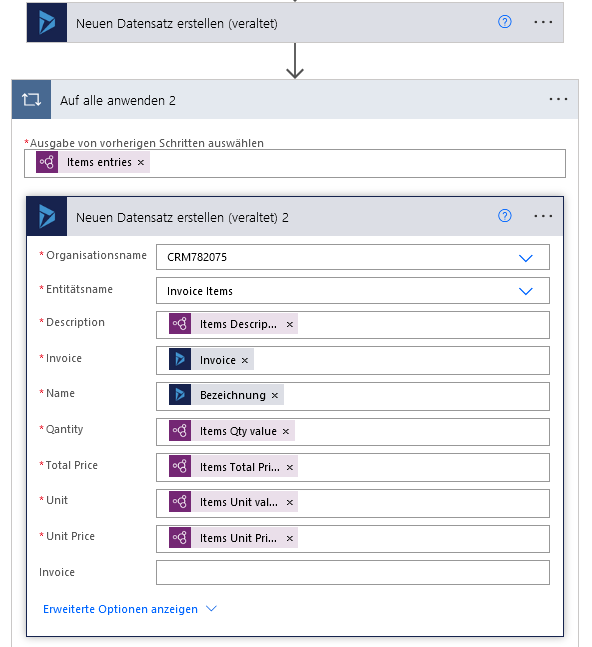
\includegraphics[scale=0.9]{sections/cloud-computing/images/power-automate-flow/insert2-dynamics-crm.png}
    \caption{Persistierung der Entitäten}
    \label{fig:persistence-entities}
\end{figure}

\ref{enum:InvoiceItemsAttributs}